\section{Virtualization}
\begin{itemize}
	\item Idea: resource usage by a single user is \textbf{under-utilized}, the \textbf{efficiency} of usage of resource is \textbf{low}.
	
	$\rightarrow$ own a machine in a shared manner $\rightarrow$ \textbf{virtualization}
	\item Definition: Virtualization is a computer architecture technology where \textbf{multiple virtual machines} are \textbf{multiplexed} in the \textbf{same hardware}. (all VMs are connected and are owners of the hardware)
	\item Goal:
	\begin{itemize}
		\item enhance resource sharing, \textbf{improve} machine \textbf{efficiency}
		\item able to replace and upgrade hardware \textbf{on the fly}, \textbf{without interrupting the running program or rebooting}.
		\item reduce down time
		\item \textbf{faster provisioning} of multiple machines 
	\end{itemize}
	\item Modes of operation:
	\begin{itemize}
		\item \textbf{kernel mode}: higher privilege
		\begin{itemize}
			\item OS allows execution of \textbf{all CPU instructions}
			\item kernel codes \textbf{don't execute in user mode}.
			\item execute in \textbf{superuser/supervisor} privilege. 
		\end{itemize}
		
		\item \textbf{user mode}:
		\begin{itemize}
			\item OS allows execution of \textbf{few CPU instructions}
			\item if user applications have to execute \textbf{privileged instructions}, they \textbf{ask kernel} to execute. 
			\item execute in user privilege.
		\end{itemize}
	\end{itemize}
\end{itemize}

\subsection{Technology for Virtualization: Hypervisors}
A \textbf{hypervisor} (or virtual machine monitor, VMM) is a kind of emulator; 
it is computer software, firmware or hardware that \textbf{creates and runs virtual machines}. 
A \textbf{computer on which a hypervisor runs} one or more virtual machines is called a \textbf{host machine}, and \textbf{each virtual machine} is called a \textbf{guest machine}. 


The hypervisor \textbf{presents the guest operating systems with a virtual operating platform and manages the execution of the guest operating systems}. Multiple instances of a variety of operating systems may \textbf{share the virtualized hardware resources}: for example, Linux, Windows, and macOS instances can all run on a single physical x86 machine. 


This contrasts with operating-system-level virtualization, where all instances (usually called containers) must share a single kernel, though the guest operating systems can differ in user space, such as different Linux distributions with the same kernel.

\subsubsection{Bare-Metal Hypervisor}
\begin{itemize}
	\item runs \textbf{directly} on \textbf{host's hardware} -- Ring 0
	\item Guest OS operates at Ring 1
	\item provides \textbf{almost full isolation} to the users. All Guest OSs are \textbf{independent} and are owner of the hardware. VMM \textbf{controls the hardware and to manages resource allocation to guest OSs}.
	\item Use-case: Hyper-V, ESX, Xen
	
\end{itemize}

\subsubsection{Hosted Hypervisor}
\begin{itemize}
	\item \textbf{runs on a conventional OS} just as other computer programs
	\item abstracts guest OSs from the host OS. 
	\item Use-case: VMware player, VMware workstation, VirtualBox
\end{itemize}

\begin{figure}[H]
	\centering
	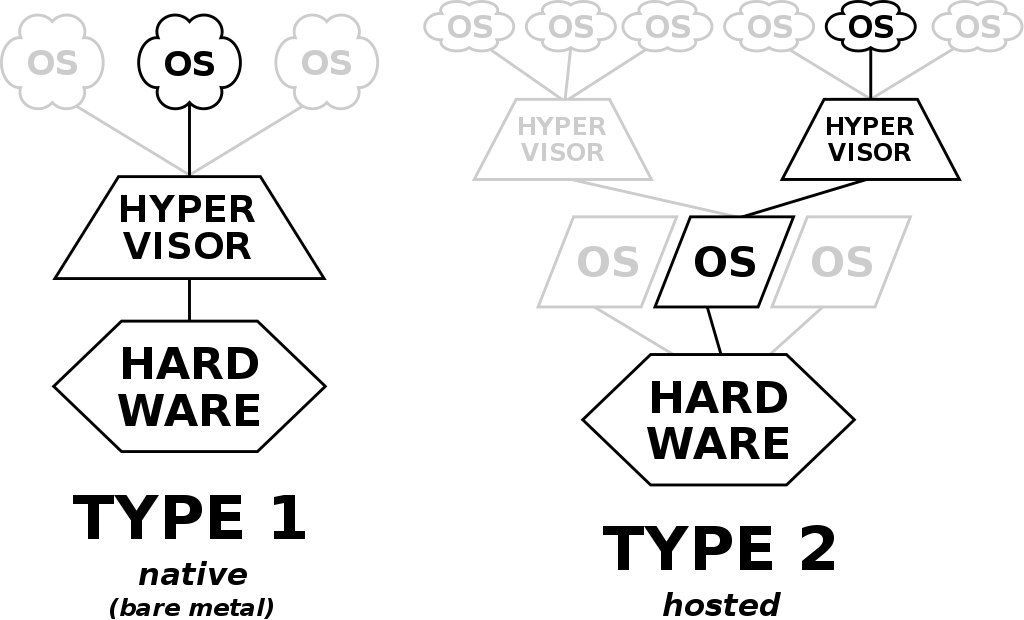
\includegraphics[width=0.65\textwidth]{hypervisor.png}
\end{figure}

\subsection{Full Virtualization}
\begin{itemize}
	\item for \textbf{any guest OS without any modifications} 
	\item VMM works in Ring 0, guest OSs work in Ring 1  -- Bare-metal hypervisor
	\item Problem: \textbf{execution error} of privilege instructions from guest OS being in \textbf{lower ring} (Ring 1)
	\begin{itemize}
		\item Solution: VMM intercepts such error and \textbf{emulates} the instructions \textbf{on the fly}
		
		$\rightarrow$ not all instructions are trapped.
		
		\item Solution: a \textbf{binary translator}, which overrides these privileged instructions and places them in translation cache. 
	\end{itemize}
	\item Consequences:
	\begin{itemize}
		\item system calls: takes \textbf{10 times more cycles} compared to no hypervisor, because \textbf{fault message} are issued, translated and executed \textbf{for every system call}. 
		
		\item I/O virtualization: major issue. \textbf{more I/Os} due to more CPUs (guest computers) but I/O chipset \textbf{can't be easily extended}
		
		
		\item memory virtualization: 2-stage mapping process with VMM.
		\begin{itemize}
			\item program's memory addresses $\rightarrow$ virtual physical memory (on VMM) $\rightarrow$ real physical memory
			\item VMM maintains a \textbf{shadow page table}, this process takes \textbf{3 to 400 more cycles} than without VMM.
		\end{itemize}
		
		
	\end{itemize}
	

\end{itemize}

\subsection{Paravirtualization}
\begin{itemize}
	\item guest OS needs to be \textbf{modified at source code level}. Information is given in prior in code, that if such instruction is being executed, it needs to go directly to the VMM instead of the hardware. 
	
	$\rightarrow$ no execution error because of ring privilege. $\rightarrow$ no trapping or binary translation needed 
	
	\item Hypervisor provides \textbf{interface} to accommodate critical kernel operations (memory management, interrupt handling)
	\item Advantages:
	\begin{itemize}
		\item runtime changes are avoided. (no on-the-fly modification)
		\item unnecessary trapping of critical instruction avoided (modified in code)
		\item lower virtualization overhead
	\end{itemize}
	Disadvantages:
	\begin{itemize}
		\item a modified guest OS needed when changing machines.
	\end{itemize}
	
\end{itemize}

\subsection{Hardware-assisted Virtualization}
\begin{itemize}
	\item Idea: enables efficient full virtualization using \textbf{help from hardware capabilities}, primarily from the host processors. 
	
	$\rightarrow$ a processor extension is introduced in a \textbf{higher priority layer} -- Root mode privilege level with VMM.
	
	\item Guest OS now operates at \textbf{Ring 0} and can execute all critical instructions
\end{itemize}

\begin{figure}[H]
	\centering
	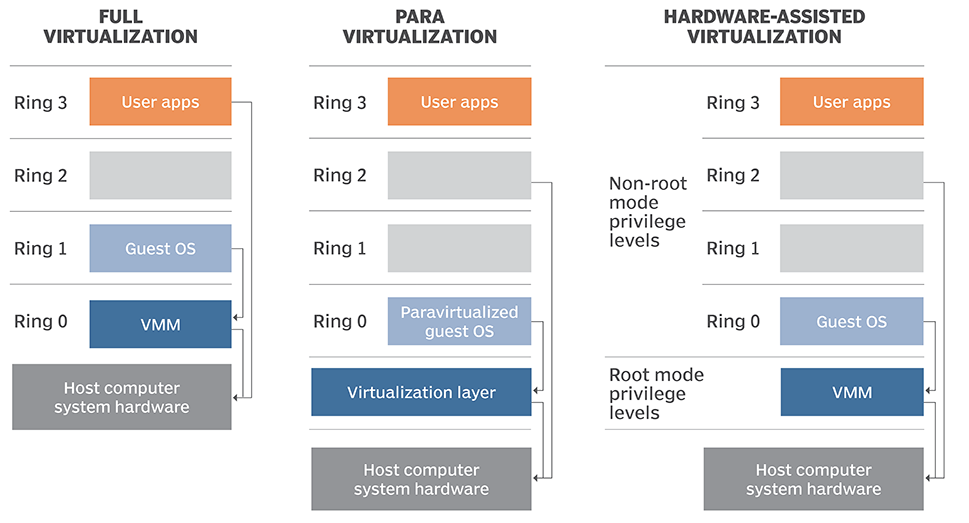
\includegraphics[width=0.7\textwidth]{virtualization.png}
\end{figure}

\subsection{OS-Level Virtualization}
\begin{itemize}
	\item Idea: 
	\begin{itemize}
		\item disadvantages of hypervisor-based virtualization: OS dependent, not scalable, not portable, slow deployment. 
		\item higher scalability required in application.  
	\end{itemize}
	$\rightarrow$ \textbf{OS-Level virtualization}
	\item VMM is \textbf{on top of host OS}
	\item building blocks: linux kernel features
	\begin{itemize}
		\item \textbf{namespaces}: \textbf{limit the views}, wrap a group of resources for limited access, managed using APIs
		\begin{itemize}
			\item PID: create another set of PID
			\item cgroup: new views to root directories
			\item network: new views to network resources
		\end{itemize}
		\item \textbf{cgroups}: control groups, \textbf{limits the applications to a specific set of resources}
		\begin{itemize}
			\item memory cgroup: memory resource controller, isolates the memory behavior of a group of task from others. when memory exceeds, running processes will be killed.
			\item others: cpu, blkio, cpuset, devices, freezer cgroup
		\end{itemize}
		
	\end{itemize}
	\item \textbf{Container}: 
	\begin{itemize}
		\item allows multiple \textbf{isolated} linux systems of same kind on a single host OS.
		\item resources are \textbf{isolated in a container} for each user.
		\item it utilizes \textbf{cgroups and namespaces} to limit the views and resources of each container.
		\item Use-case: \textbf{Docker}
		\item Advantages:
		\begin{itemize}
			\item runtime isolation: isolates different runtime environments based on application requirement
			\item cost-efficiency: no creation of entire virtual OS for each user.
			\item easy portability of containers
			\item high scalability, easy replication of containers across environments
			\item faster deployment: layer-concept, only new layers/updated layers are built. 
			 
		\end{itemize}
	\end{itemize}
	\begin{figure}[H]
		\centering
		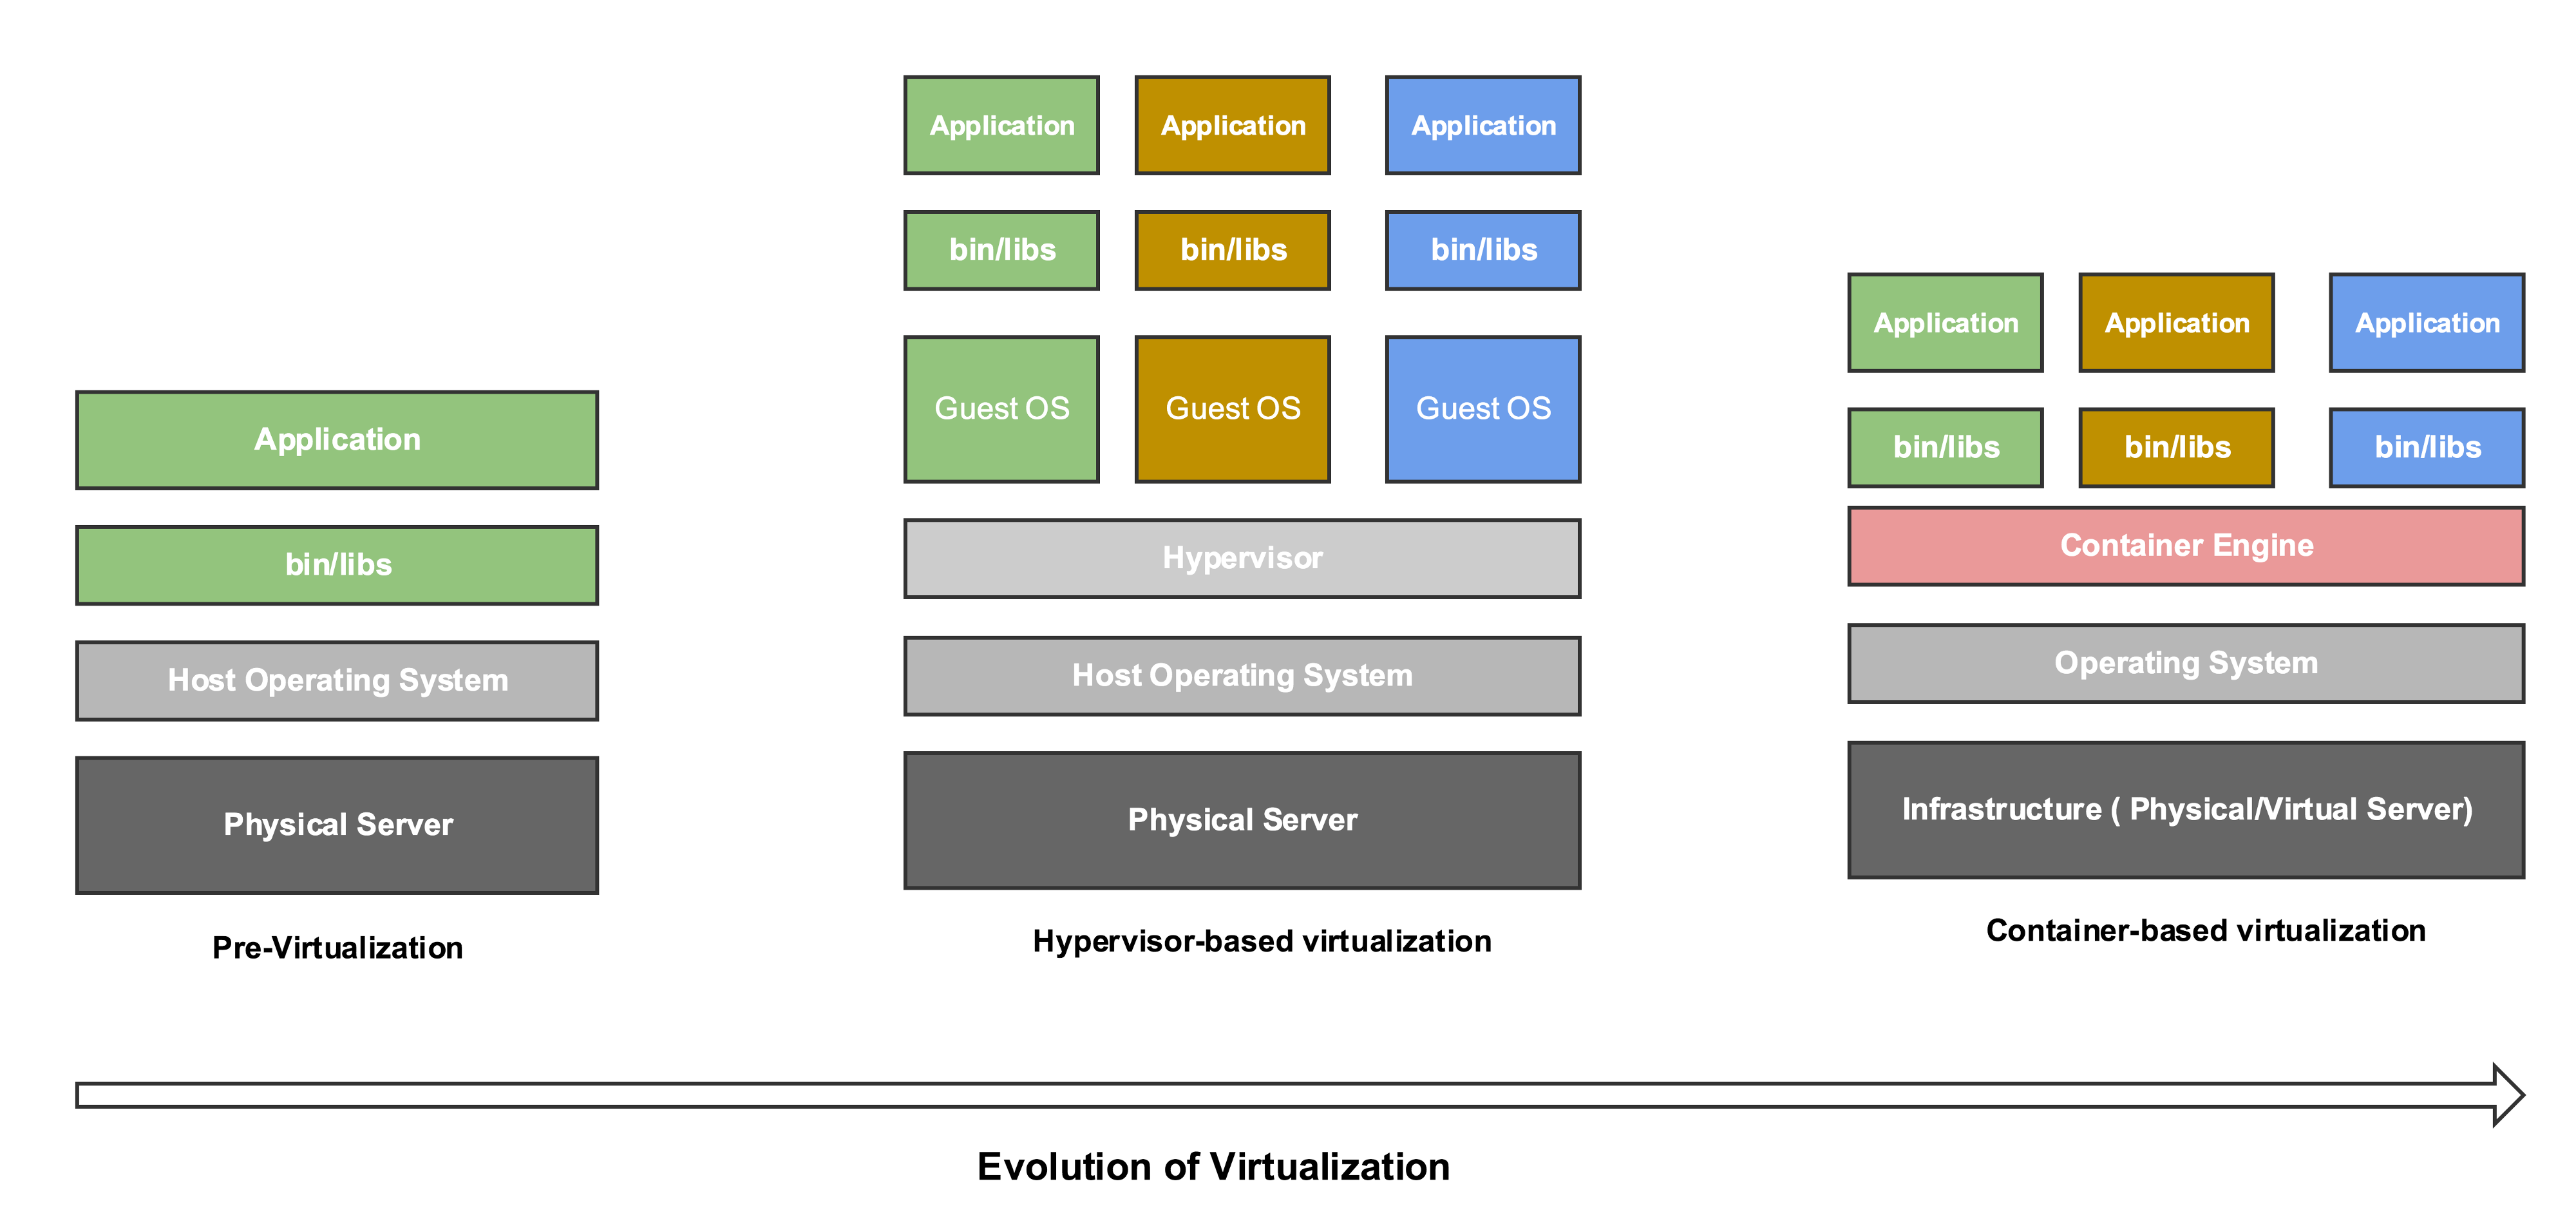
\includegraphics[width=\textwidth]{container.png}
	\end{figure}
\end{itemize}

